\pagestyle{empty}				% no header or footers
\chapter{Paper I}
\vfil\null
\huge{\textbf{Brief communication: Growth and decay of an ice stupa in alpine conditions – a simple model driven by energy-flux observations over a glacier surface}}

\bigskip
\large{
Oerlemans, J., S. Balasubramanian, C. Clavuot, and F. Keller. The Cryosphere 15, no. 6 (2021): 3007–12. doi:10.5194/tc-15-3007-2021.
  }

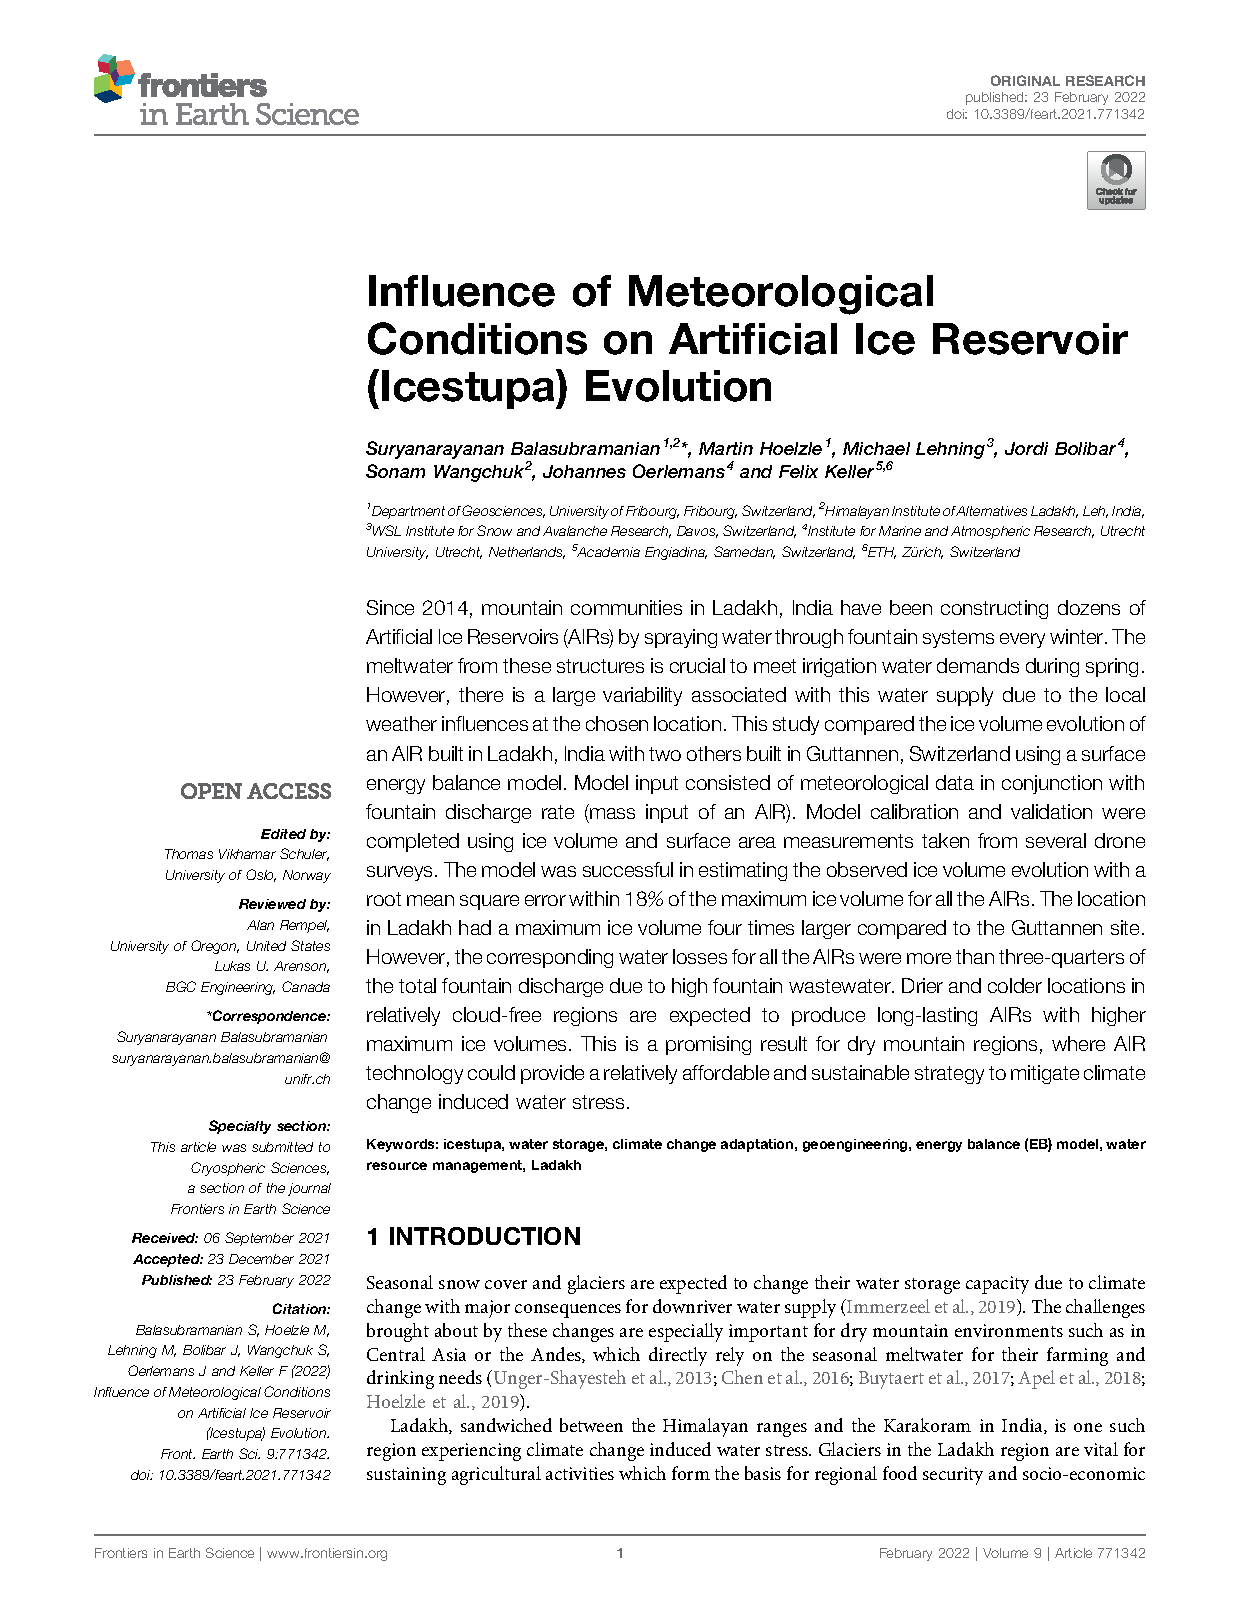
\includepdf[pages=-,pagecommand={},width=\paperwidth, scale=10]{content/papers/paperI.pdf}

\chapter{Paper II}
\vfil\null
\huge{\textbf{Influence of Meteorological Conditions on Artificial Ice Reservoir (Icestupa) Evolution}}

\bigskip
\large{Balasubramanian, S., Hoelzle, M., Lehning, M., Bolibar, J., Wangchuk, S.,
  Oerlemans, J., and Keller, F. \par  Frontiers in Earth Science 9 (February 23, 2022): 771342.
doi:10.3389/feart.2021.771342.}

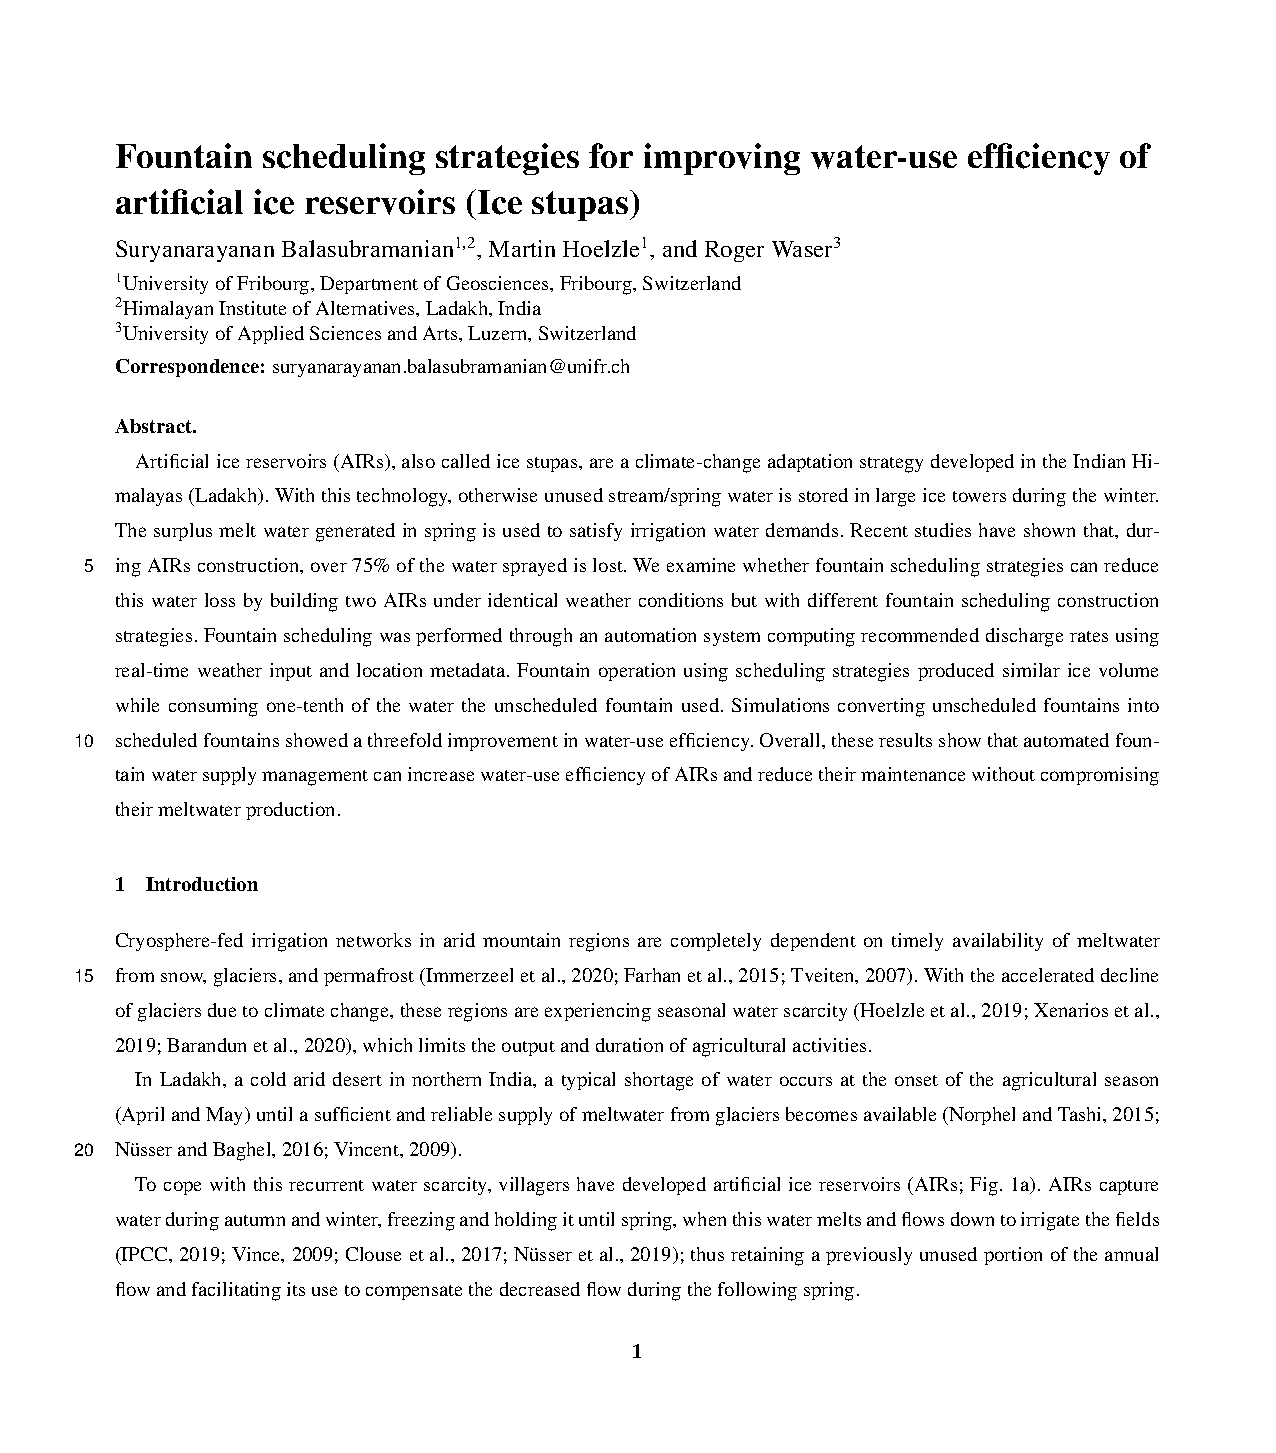
\includepdf[pages=-,pagecommand={},width=\paperwidth, scale=10]{content/papers/paperII.pdf}

\chapter{Paper III}
\vfil\null
\huge{\textbf{Improving water-use efficiency of artificial ice reservoirs (Icestupas) through weather-sensitive fountain scheduling
strategies}}

\bigskip
\large{Balasubramanian, S., Hoelzle, M., and Waser, R. \par  Frontiers in Earth Science 9 (February 23, 2022): 771342. doi:10.3389/feart.2021.771342.}

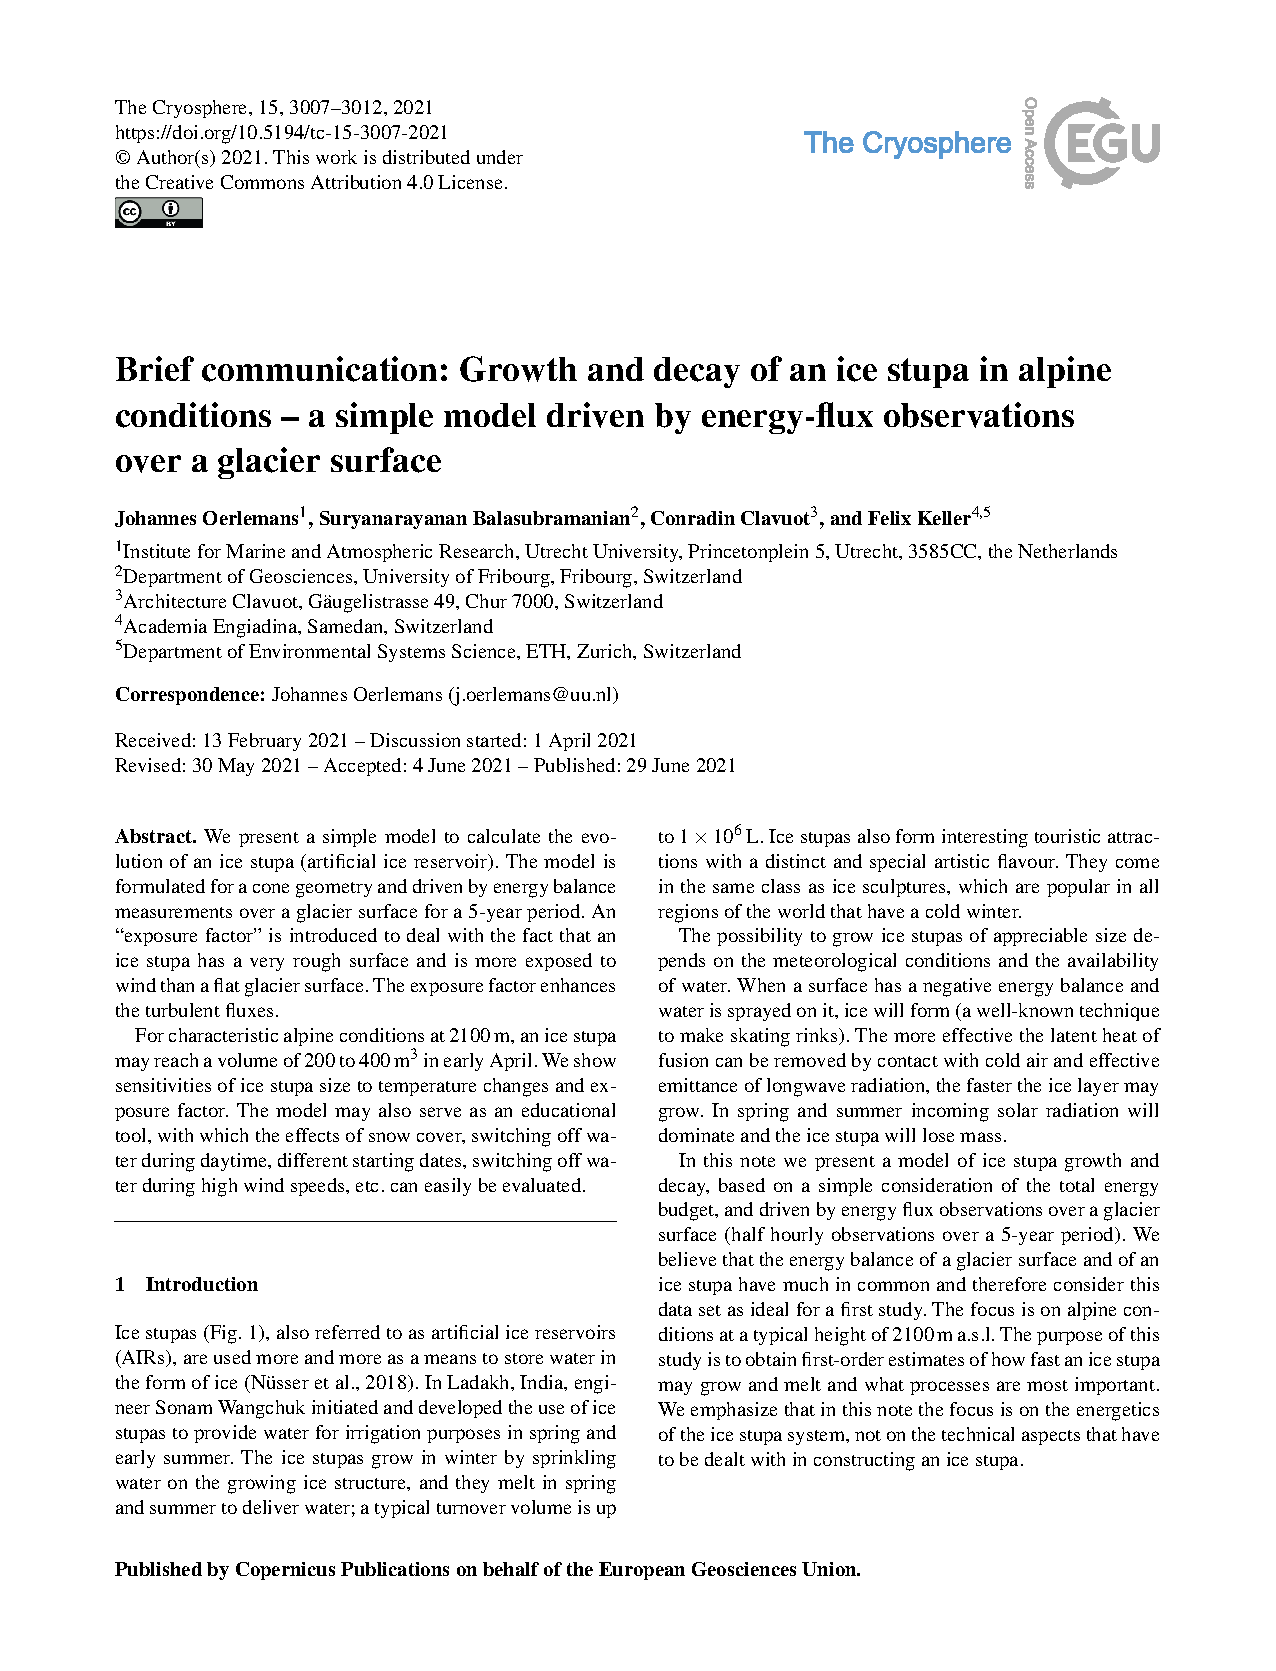
\includepdf[pages=-,pagecommand={},width=\paperwidth, scale=10]{content/papers/paperIII.pdf}

